\documentclass[border=10pt]{standalone}
\usepackage{amssymb}
\usepackage{amsmath}
\usepackage{tikz}
\usetikzlibrary{positioning, shapes.geometric, calc}

\definecolor{cnavy}{HTML}{0E2747}
\definecolor{corange}{HTML}{E8573F}
\definecolor{cgreen}{HTML}{3B9B6D}
\definecolor{cslate}{HTML}{5B6680}
\definecolor{cmuted}{HTML}{9B9484}
\definecolor{ccream}{HTML}{FAFAF6}

\begin{document}
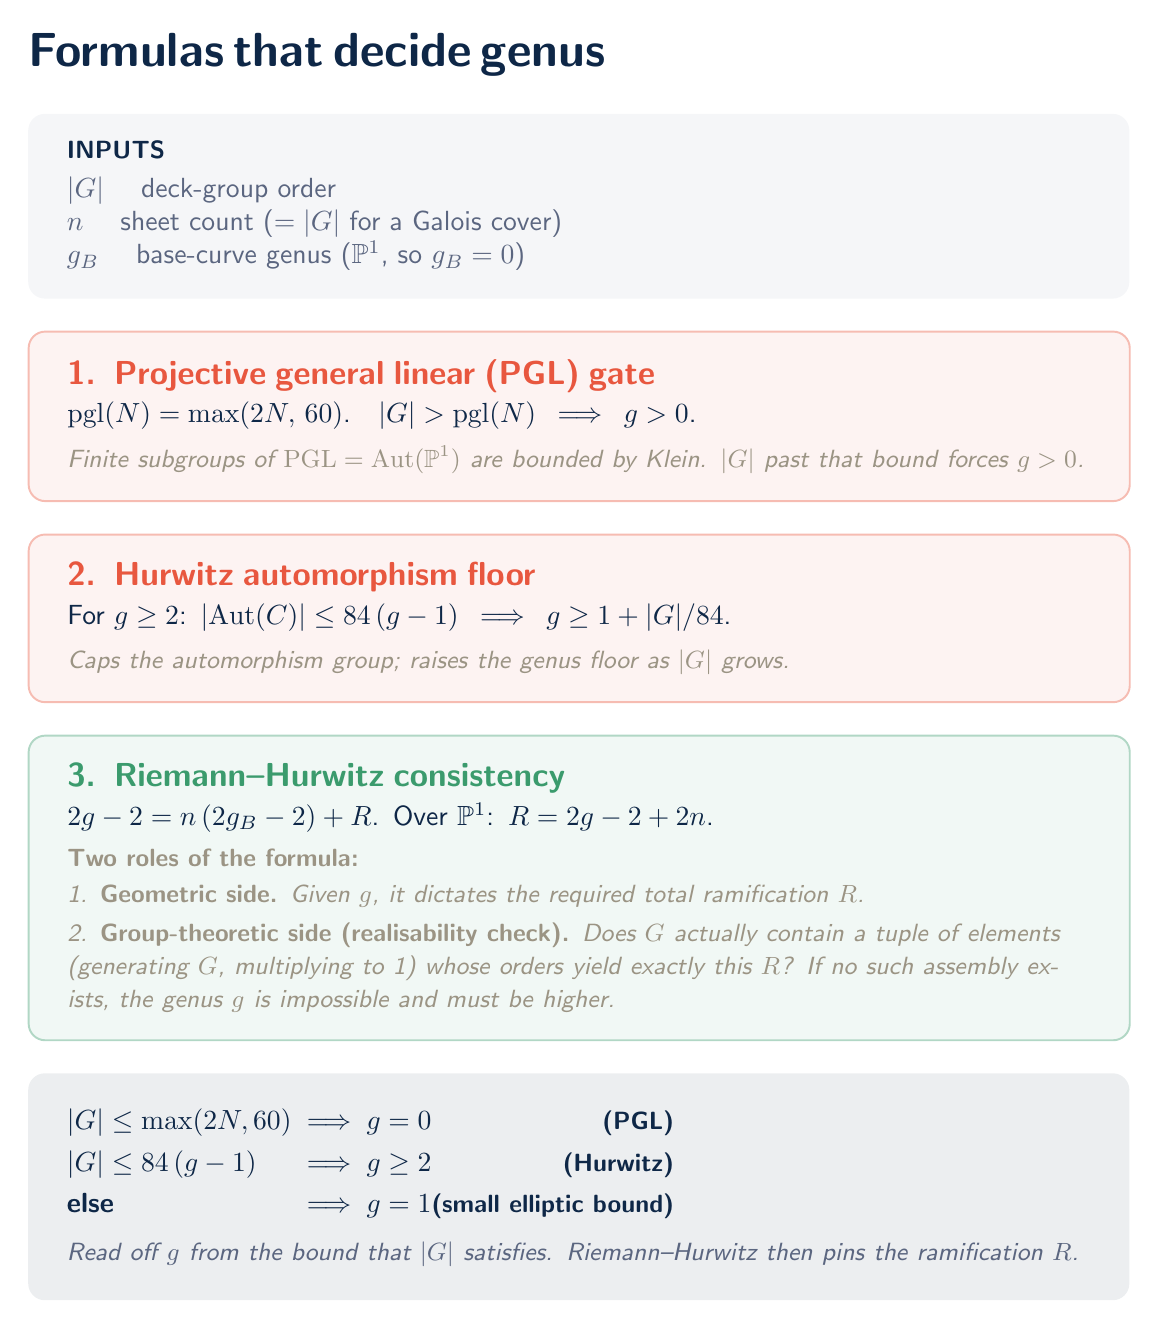
\begin{tikzpicture}[
  font=\sffamily,
  every node/.append style={anchor=north west, align=left},
  headcard/.style={
    rectangle,
    inner xsep=0pt, inner ysep=2pt,
    text width=13.6cm
  },
  inputscard/.style={
    rectangle, rounded corners=6pt,
    fill=cnavy!4,
    inner xsep=14pt, inner ysep=10pt,
    text width=13cm, draw=none
  },
  formulacardO/.style={
    rectangle, rounded corners=6pt,
    fill=corange!7, draw=corange!40, line width=0.7pt,
    inner xsep=14pt, inner ysep=10pt,
    text width=13cm
  },
  formulacardG/.style={
    rectangle, rounded corners=6pt,
    fill=cgreen!7, draw=cgreen!40, line width=0.7pt,
    inner xsep=14pt, inner ysep=10pt,
    text width=13cm
  },
  combinecard/.style={
    rectangle, rounded corners=6pt,
    fill=cnavy!8,
    inner xsep=14pt, inner ysep=12pt,
    text width=13cm, draw=none
  }
]

\node[headcard] (hd) at (0, 0) {%
  {\bfseries\LARGE\color{cnavy} Formulas that decide genus}
};

\node[inputscard, below=4mm of hd.south west, anchor=north west] (in) {%
  {\bfseries\small\color{cnavy} INPUTS}\\[2pt]
  \color{cslate}\normalsize
  $|G|$\quad{} deck-group order \\
  $n$\quad{} sheet count ($= |G|$ for a Galois cover)\\
  $g_B$\quad{} base-curve genus ($\mathbb{P}^1$, so $g_B = 0$)
};

\node[formulacardO, below=4mm of in.south west, anchor=north west] (f1) {%
  {\bfseries\large\color{corange} 1.\enspace Projective general linear (PGL) gate}\\[2pt]
  \color{cnavy}\normalsize
  $\mathrm{pgl}(N) = \max(2N,\, 60)$.\quad
  $|G| > \mathrm{pgl}(N)\enspace \Longrightarrow\enspace g > 0$.
  \\[4pt]
  \itshape\color{cmuted}\small
  Finite subgroups of $\mathrm{PGL} = \mathrm{Aut}(\mathbb{P}^1)$ are bounded by Klein. $|G|$ past that bound forces $g > 0$.
};

\node[formulacardO, below=4mm of f1.south west, anchor=north west] (f2) {%
  {\bfseries\large\color{corange} 2.\enspace Hurwitz automorphism floor}\\[2pt]
  \color{cnavy}\normalsize
  For $g \geq 2$:\enspace
  $|\mathrm{Aut}(C)| \leq 84\,(g-1)\enspace \Longrightarrow\enspace g \geq 1 + |G|/84$.
  \\[4pt]
  \itshape\color{cmuted}\small
  Caps the automorphism group; raises the genus floor as $|G|$ grows.
};

\node[formulacardG, below=4mm of f2.south west, anchor=north west] (f3) {%
  {\bfseries\large\color{cgreen} 3.\enspace Riemann\nobreakdash--Hurwitz consistency}\\[2pt]
  \color{cnavy}\normalsize
  $2g - 2 = n\,(2 g_B - 2) + R$.\enspace
  Over $\mathbb{P}^1$:\enspace $R = 2g - 2 + 2n$.
  \\[4pt]
  \color{cmuted}\small
  {\bfseries Two roles of the formula:}\\[2pt]
  \itshape
  1.\enspace {\bfseries\upshape Geometric side.}\itshape\enspace Given $g$, it dictates the required total ramification $R$.\\[2pt]
  2.\enspace {\bfseries\upshape Group-theoretic side (realisability check).}\itshape\enspace Does $G$ actually contain a tuple of elements (generating $G$, multiplying to 1) whose orders yield exactly this $R$? If no such assembly exists, the genus $g$ is impossible and must be higher.
};

\node[combinecard, below=4mm of f3.south west, anchor=north west] (cb) {%
  \color{cnavy}\bfseries
  \begin{tabular}{@{}l@{\enspace}c@{\enspace}l@{\hfill}r@{}}
    $|G| \leq \max(2N, 60)$ & $\Longrightarrow$ & $g = 0$ & {\small (PGL)} \\[3pt]
    $|G| \leq 84\,(g-1)$    & $\Longrightarrow$ & $g \geq 2$ & {\small (Hurwitz)} \\[3pt]
    $\text{else}$           & $\Longrightarrow$ & $g = 1$ & {\small (small elliptic bound)}
  \end{tabular}
  \\[6pt]
  \mdseries\itshape\color{cslate}\small
  Read off $g$ from the bound that $|G|$ satisfies. Riemann\nobreakdash--Hurwitz then pins the ramification $R$.
};

\end{tikzpicture}
\end{document}
